\documentclass[10pt,a4paper,twocolumn]{article}
\usepackage[dvipdfmx]{graphicx}
\usepackage[dvipdfmx]{hyperref}
\begin{document}

\title{Experiment of training Full Ternary Weights Network(FTWN) with darknet YOLO}
\author{Kenji Ogura}
\date{}
\maketitle

\section{Abstract}
Generally ternarizing weights of model needs retraining after ternarization of weights.
To reduce accuracy damage by ternarization I propose the staged training method(STM) for full ternary weights network(FTWN).
At STM retraining and ternarizing pair consist of 4 pairs of Ternarizing and retraining to avoid local minumum problem.
STM widens ternarizing layers until full ternary weights step by step.
To confirm effect of STM at experiment I customize darknet framework to support weights ternarizing in convolutional layer and integrate training algorithm in it.
I train yolov2 and yolov3 models on customized darknet framework with VOC dataset 2012 and 2007 and test with VOC 2007 and get mAP as results.
Full ternarized yolov2 with STM perform 73.82\% mAP against full precision's 76.85\% mAP.
Full ternarized yolov3 with STM perform 71.26\% mAP against full precision's 75.54\% mAP.

\section{Related works}

\begin{itemize}
\item
 Training algorithm refer to "Alorithm 1" in "XNOR-Net: ImageNet Classification Using BinaryConvolutional Neural Networks"\cite{Rastegari2015XNORNetIC}
\item
 Equation to Ternarize weights with scale factor Wl refer to "equation (3)" in "Ternary weight networks"\cite{Li2016TernaryWN}
\end{itemize}

Generally the inference task using full ternary weights -1,0,+1 with scaling factor Wl is considered as low accuracy than full precision weights.
However for mobile device such as raspberryPI small weights will be efficient one of choices.
Some quantinization methods for model weights are proposed now such as FP16, bfloat, fixed point 16bits, 8bit, ternary 2bits and XNor 1bit too.
I consider that re-training after quatinization of weights is needed.
In this paper I propose Staged Trainiing Method(STM) for full ternary weights network and show the result as mAP.

\section{Staged training method}
In this paper I propose the staged training for yolov2-voc.cfg\cite{redmon2016yolo9000}, yolov3-voc.cfg\cite{yolov3} on Darknet website.
You can get full ternarized weights within 3 points accuracy drops for yolov2, within 4.5 points accuracy dorops for yolov3 using this method.
2bits ternary weights representaion may be x16 smaller than 32bit floating point.

STM generates Ternarized weights for yolov2-voc, yolov3-voc.
This method sprits a training step into 4 stages. Staging Plan is below,

\begin{itemize}
\item Stage-0 : few layers without around of detector are ternarized(M0)
\item Stage-1 : 40\% of all layers are ternarized(M1)
\item Stage-2 : 90\% of all layers are ternarized(M2)
\item Stage-3 : full ternarized(M3)
\end{itemize}

Each stages import weights from previous stage, such as stage-2 weights from stage-1.
However stage-0(M0) imports usual full precision weights.
Figure.1 shows staging for yolov2-voc.cfg into 4 training stages, and Figure.2 for yolov3-voc.cfg.
On each figures 'F' denote full precision weights and 'T' denotes ternarized weights.
To estimate this staged training method I implement ternary keyword for each convolution layer in cfg file like 'ternary=1' and I also support ternarizing weights function and ternarized weights memory area in darknet framework.
To avoid local minimun problem via training ternarized model I sprit training into some steps.

\begin{figure}
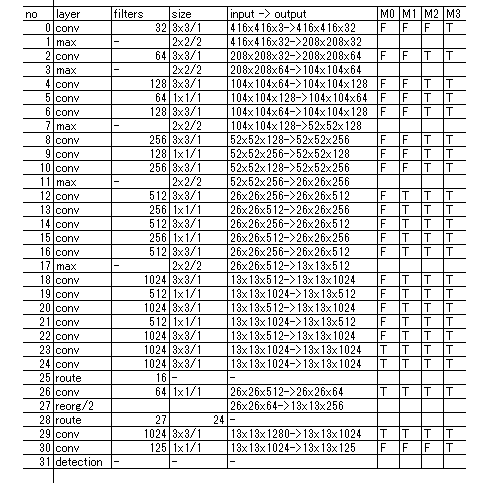
\includegraphics[width=8cm]{yolov2-voc_Stages.png}
\caption{Staging for yolov2-voc.cfg}
\end{figure}

\begin{figure}
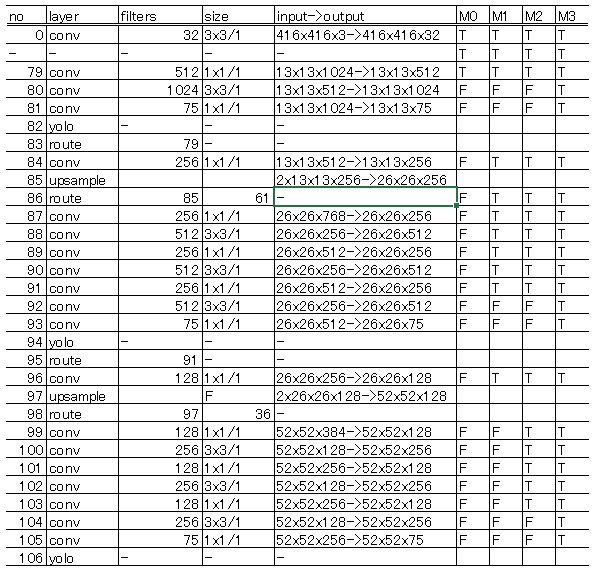
\includegraphics[width=8cm]{yolov3-voc_Stages.png}
\caption{Staging for yolov3-voc.cfg}
\end{figure}

I trained yolov2-voc.cfg on 4 jobs, and checked each loss curves on Excell graph.
And I use \href{https://github.com/AlexeyAB/darknet}{AlexeyAB darknet} to get mAP of experiments.

\section{Result of Training}

Tables denote the result of my staged training.
VOC 2012, 2007 Dataset is used with training and VOC 2007 for estimation of mAP.

\begin{table}[htbp]
 \centering
 \begin{tabular}{c|c|c|l}
  Stage & mAP & IOU & comments \\ \hline\hline
  -        & 76.85 & 54.67 & official Weights \\ \hline
  M0       & 77.09 & 57.04 & -                \\ \hline
  M1       & 76.44 & 56.18 & -                \\ \hline
  M2       & 75.06 & 57.71 & -                \\ \hline
  M3       & 73.82 & 54.90 & full ternary     \\ \hline\hline
 \end{tabular}
 \caption{result regard to yolov2}
 \label{tb:yolov2}
\end{table}

In Table.1 Iteration 41000(2000/class), steps x0.1 80\% 90\%, lr=0.001 at all stages

\begin{table}[htbp]
 \centering
 \begin{tabular}{c|c|c|l}
  Stage & mAP & IOU & comments \\ \hline\hline
  -        & 75.54 & 62.78 & FT from darknet53.conv.75 \\ \hline
  M0       & 75.02 & 63.04 & -                \\ \hline
  M1       & 73.69 & 63.75 & -                \\ \hline
  M2       & 73.76 & 63.54 & -                \\ \hline
  M3       & 71.26 & 61.61 & full ternary     \\ \hline\hline
 \end{tabular}
 \caption{result regard to yolov3}
 \label{tb:yolov3}
\end{table}

In Table.2 Iteration 100400(5000/class), steps x0.1 80\% 90\%, lr=0.001 at M0 and M1
Iteration 60400(3000/class), steps x0.1 80\% 90\%, lr=0.001 at M2 and M3.

\section{Conclusion}

If your applications using object detection task requires speed but not accuracy you can use full ternary weights network.
To get efficient ternary weights you can use staged training method in this paper.
Ternary weights is x16 smaller than fp32 representation.
Full ternary weights network performs accuracy within 4.5\% mAP drops with yolov2 or yolov3 network on darknet framework.

\begin{thebibliography}{1}

\bibitem{Li2016TernaryWN}
Fengfu Li and Bin Liu.
\newblock Ternary weight networks.
\newblock {\em ArXiv}, abs/1605.04711, 2016.

\bibitem{Xu2018TrainingAB}
Jiaolong Xu, Peng Wang, Haishun Yang, and Antonio.Lpez.
\newblock Training a binary weight object detector by knowledge transfer for
  autonomous driving.
\newblock {\em 2019 International Conference on Robotics and Automation
  (ICRA)}, pages 2379--2384, 2018.

\bibitem{Rastegari2015XNORNetIC}
Mohammad Rastegari, Vicente Ordonez, Joseph Redmon, and Ali Farhadi.
\newblock Xnor-net: Imagenet classification using binary convolutional neural
  networks.
\newblock {\em ArXiv}, abs/1603.05279, 2016.

\bibitem{redmon2016yolo9000}
Joseph Redmon and Ali Farhadi.
\newblock Yolo9000: Better, faster, stronger.
\newblock {\em arXiv preprint arXiv:1612.08242}, 2016.

\bibitem{yolov3}
Joseph Redmon and Ali Farhadi.
\newblock Yolov3: An incremental improvement.
\newblock {\em arXiv}, 2018.

\end{thebibliography}

\end{document}
